\chapter{Performance Evaluation}
\label{ch:evaluation}

In this section, 整理效能評估.

下面是subfigure的範例 (其實我個人不常用這個語法, 我都直接在繪圖工具上把圖片整合在一起 XD)

\begin{figure}
     \centering
     \begin{subfigure}[]{0.3\textwidth}
         \centering
         
\includegraphics[width=\textwidth]{img/fig1.png}
         \caption{figure 1}
         \label{fig:11111}
     \end{subfigure}
     \hfill
     \begin{subfigure}[]{0.3\textwidth}
         \centering
         
\includegraphics[width=\textwidth]{img/fig2.png}
         \caption{figure 2}
         \label{fig:22222}
     \end{subfigure}
     \hfill
     \begin{subfigure}[]{0.3\textwidth}
         \centering
         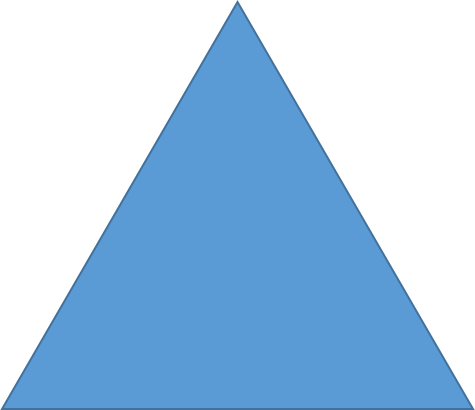
\includegraphics[width=\textwidth]{img/fig3.png}
         \caption{figure 3}
         \label{fig:33333}
     \end{subfigure}
        \caption{Three simple graphs}
        \label{fig:three graphs}
\end{figure}